In order to maintain the configuration of the constellation for a longer time, a thruster is installed in each satellite to correct the decrease in altitude due to the orbit decay. To maintain the altitude the thruster will apply a velocity increment to the satellite to change its orbit and, consequently, its altitude. This is a maneuver. It can be an impulsive maneuver, in which the velocity increment is added instantaneously, or non-impulsive, in which $\Delta$V is applied during a significant amount of time. The optimal maneuver is an impulsive one, the Hohmann transfer, a single-impulse maneuver. Hohmann has the best relation between propellant consumed and time required to do the maneuver. However, non-impulsive maneuvers like low-thrust maneuver require lower velocity increments and are less propellant-consuming.

To maintain the altitude, Astrea satellites will compute a low-thrust maneuver. However, since this is a preliminar study, the calculations will be computed for a Hohmann transfer maneuver, which is simpler and requires more propellant and greater increases of velocity. That is, by computing the velocity and propellant needed for a Hohmann maneuver, the results will be safe for a low-trust maneuver, because the late one requires less energy.

\subsubsubsection*{Orbit maintenance}
The method proposed begins when the satellite is deployed at a given height. This height will decrease due to the orbit decay, reaching a critical value, a limit altitude. Once this critical altitude is achieved, the satellite is put once again at its initial height through a Hohmann maneuver. The process is repeated several times until the satellite runs out of propellant or until it reaches its desired lifetime. All the calculations needed are developed in \cite[Chapter 4, Section 3]{annex1}.

As mentioned before, in reality the satellite will perform a low-thrust maneuver, which is more practical for an electric thruster. In this non-impulsive maneuver, the thruster is constantly providing a velocity increment to the satellite, but it is so small that the whole transfer maneuver requires a lot of time. This means that it is not necessary to wait until the satellite reaches the critical altitude. The maneuver will start when the satellite is deployed or when it reaches a given altitude (higher than the critical altitude) so that it counteracts the effect of the orbital decay.

\subsubsubsection*{Results}
The results are computed for a 3U CubeSat with an ion thruster. The characteristics of the thruster are the ones shown on table \ref{thrustspimpulse}. For more information on the thruster refer to section \ref{ch:PropulsionSystems}.

\begin{table}[h!]
\begin{center}
\begin{tabular}{ | l | l | }
\hline
Thrust & 100 $\mu$N \\ 
\hline 
Specific Impulse & 2150 s \\
\hline
\end{tabular}
\caption{Simulation Thruster Parameters}
\label{thrustspimpulse}
\end{center}
\end{table}

The first parameters to be defined are the maximum and minimum height of the orbit, mesured from the surface of the Earth. The maximum height is the altitude at which the satellite is deployed, and minimum height is the altitude at which the Hohmann transfer maneuver is applied.

Figure \ref{fig:hohmann3km} is an example of the height variation of the satellite using the Hohmann maneuver to reach the maximum height once the satellite is in the minimum height. The results of this maneuver are:

\begin{minipage}{\textwidth}
\begin{minipage}[b]{0.49\textwidth}
\centering
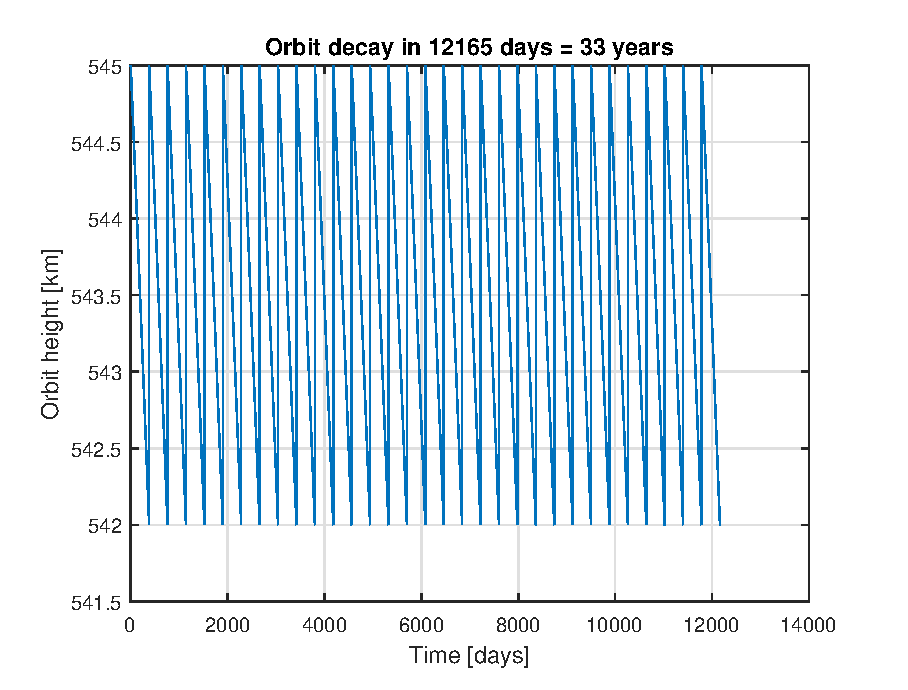
\includegraphics[scale=0.4]{ThrustersDrag/thrust3km.eps}
\captionof{figure}{Height variation of the satellite}
\label{fig:hohmann3km}
\end{minipage}
\hfill
\resizebox{7cm}{!}{
\begin{minipage}[b]{0.54\textwidth}
\centering
\begin{tabular}{ | l | l | }
\hline
Maximum height & 545 km \\
\hline
Minimum height & 542 km \\
\hline
Number of Hohmann Maneuvers & 32 \\
\hline
Maximum $\Delta$V\textsubscript{1} & 0,8237 m/s \\
\hline
Maximum $\Delta$V\textsubscript{2} & 0,8236 m/s \\
\hline
Total $\Delta$V Budget & 52,7116 m/s \\ 
\hline 
Propellant mass & 10 g \\
\hline
Lifetime of the satellite & 33,3288 years \\
\hline
\end{tabular}
\captionof{table}{Station-Keeping with Thrusters Simulation 1 Results}
\end{minipage}
}
\end{minipage}

Since the thruster used is an ion thruster, the specific impulse is big, and the mass propellant is very low. In this case, the variation of height due to the orbit decay is approximately 3 km per year, so the thruster needs to do a Hohmann maneuver per year. With only 10 g of propellant, the lifetime of the satellite is over 30 years.

Figure \ref{fig:hohmann80m} is another example of the Hohmann maneuver with the same amount of propellant but with a more restrictive range of operational heights, only 80 m. It should have the same shape as Figure \ref{fig:hohmann3km}, but since a lot of maneuvers are applied, the lines have overlapped. The characteristics of this maneuver are:

\begin{minipage}{\textwidth}
\begin{minipage}[b]{0.49\textwidth}
\centering
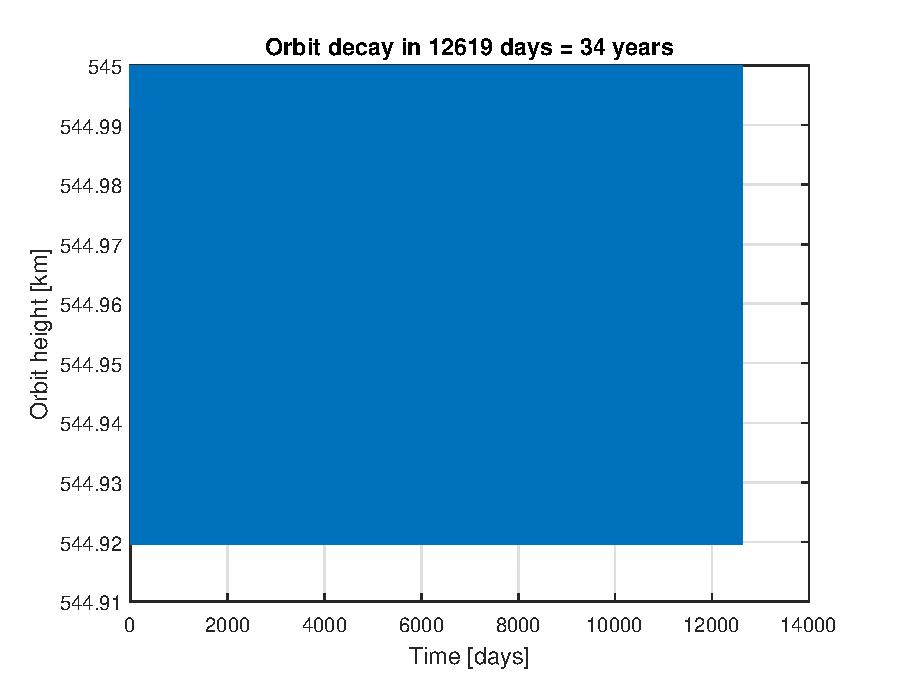
\includegraphics[scale=0.4]{ThrustersDrag/thrust80m.eps}
\captionof{figure}{Height variation of the satellite with a more restrictive minimum height}
\label{fig:hohmann80m}
\end{minipage}
\hfill
\resizebox{7cm}{!}{
\begin{minipage}[b]{0.54\textwidth}
\centering
\begin{tabular}{ | l | l | }
\hline
Maximum height & 545 km \\
\hline
Minimum height & 544,92 km \\
\hline
Number of Hohmann Maneuvers & 1200 \\
\hline
Maximum $\Delta$V\textsubscript{1} & 0,0221 m/s \\
\hline
Maximum $\Delta$V\textsubscript{2} & 0,0221 m/s \\
\hline
Total $\Delta$V Budget & 52,7570 m/s \\ 
\hline 
Propellant mass & 10 g \\
\hline
Lifetime of the satellite & 34,5726 years \\
\hline
\end{tabular}
\captionof{table}{Station-Keeping with Thrusters Simulation 2 Results}
\end{minipage}
}
\end{minipage}

Comparing these results with the previous ones, it can be seen that with a more restrictive range of heights, the lifetime of the satellite is practically the same. The velocity increments are lower because the difference in the heights is extremely low, but at the same time, the satellite reaches before the minimum height and the number of maneuvers needed to maintain the satellite in this range are many more than on the other case. Since the $\Delta$V budget is practically the same in both cases, it can be assured that the only difference between them is the number of maneuvers computed.

As mentioned earlier, the results obtained are for a Hohmann maneuver when in reality the satellite will compute a low-thrust maneuver, that requires less velocity increments and less propellant. In conclusion, taking into account these results, it can be stated that the lifetime of the satellite will not be determined by its orbit decay but for the failure of its systems or other external causes. It can also be assured that the satellite is capable of carrying enough propellant to maintain its altitude and to compute other maneuvers if necessary.